%------------------------------------------------------------------------------------------------
%PAGINA 1 INTRODUCCION
\thispagestyle{plain}
\begin{center}
{\Large \textbf{CAPÍTULO 1}}\\[3\baselineskip]
{\LARGE \textbf{SISTEMA}}
\end{center}

\vspace{1cm}

\noindent
{\fontsize{14}{16}\selectfont
Toda ciencia estudia sistemas de algún tipo, ya sean naturales (físicos, químicos, biológicos o sociales) o artificiales (técnicos). Además, la mayoría de las ciencias no estudia otra cosa que sistemas. Así, la biología estudia biosistemas, la sociología sociosistemas y la tecnología tecnosistemas. La física parece ser la única ciencia que investiga no solo sistemas —como los átomos y los campos a gran escala—, sino también cosas supuestamente simples o elementales, como los electrones y los fotones. Aun así, los físicos reconocen que cada una de esas cosas básicas es un componente de algún sistema.

Hasta hace poco, cada tipo de sistema se estudiaba por separado. Hace unas cuatro décadas, varios especialistas unieron esfuerzos para emprender diversas iniciativas interdisciplinarias, como la investigación operativa y la cibernética.  
El éxito de estas empresas sugirió a algunos investigadores que era posible un enfoque unificado para los problemas de distintos campos. Señalaron que:  
(a) existen ciertos conceptos y principios estructurales que parecen aplicarse a sistemas de muchos tipos, y  
(b) hay algunas estrategias de modelado —en particular el enfoque del \textit{espacio de estados}— que parecen funcionar en todas partes.

La disciplina que pretende desarrollar tal enfoque unificado suele llamarse \textit{``teoría general de sistemas''} (Bertalanffy, 1950, 1958; Boulding, 1956). Paradójicamente, no se trata de una sola teoría, sino de todo un conjunto de teorías —teoría de autómatas, teoría de sistemas lineales, teoría de control, teoría de redes, dinámica lagrangiana general, etc.— unificadas por un marco filosófico (Bunge, 1974c, 1977c). Llamaremos \textit{sistemismo} a este conjunto de teorías que se centran en las características estructurales de los sistemas y, por tanto, pueden atravesar las barreras —en gran parte artificiales— entre las disciplinas.

El sistemismo tiene dos motivaciones relacionadas: una cognitiva y otra práctica.  
La motivación cognitiva o teórica del sistemismo es, por supuesto, el deseo de descubrir similitudes entre sistemas de todo tipo a pesar de sus diferencias específicas —por ejemplo, entre los sistemas de control de temperatura corporal y los termostatos de los hornos—.  
La motivación práctica del sistemismo es la necesidad de enfrentarse a los sistemas enormes y multifacéticos característicos de las sociedades industriales —como las redes de comunicación, las fábricas, los hospitales y los ejércitos—. Esta complejidad, en particular la variedad de componentes de dichos sistemas, rompe las fronteras tradicionales entre disciplinas y exige un enfoque interdisciplinario.
}

%------------------------------------------------------------------------------------------------
%PAGINA 2
\newpage

\pagestyle{fancy}
\begin{center}
{\fontsize{16}{18}\selectfont \textbf{CAPÍTULO 1}}\\[0.8cm]
\end{center}

\vspace{0cm}

{\fontsize{13}{15}\selectfont
Obsérvese la diferencia entre el científico, ingeniero o científico social convencional, por un lado, y el “especialista” en sistemas (en realidad un generalista), por el otro. Mientras que los primeros practican o aplican alguna ciencia particular, el experto en sistemismo resta importancia a la física (química, biología o sociología) de sus sistemas, centrándose en cambio en su estructura y comportamiento.

Además, se interesa especialmente en duplicar o imitar (modelar o simular) el comportamiento de un sistema dado (por ejemplo, una persona) mediante otro de tipo diferente (por ejemplo, un autómata de reconocimiento de patrones). Esto es válido no solo para el matemático que adopta el sistemismo como un pretexto honorable para jugar con estructuras abstractas sin una preocupación seria por los problemas prácticos de la ingeniería o la gestión; también se aplica al sistemista que busca resolver problemas concretos, como modelar y simular un sistema de pastoreo o una universidad.

El método empleado por el teórico de sistemas es el modelado matemático y la verificación experimental (o al menos computacional) de los modelos de sistemas. Ambos forman parte, por supuesto, del método científico. Lo peculiar del modo en que procede el experto en sistemismo es que, lejos de incorporar leyes específicas (por ejemplo, químicas) en su modelo, busca construir una \textit{caja negra}, una \textit{caja gris} o un modelo cinemático libre de detalles sobre los materiales que componen el sistema, lo suficientemente general como para abarcar algunos de los aspectos globales de la organización y del comportamiento del sistema en algunos de sus niveles.  
Así, el método científico se da por supuesto: lo que se enfatiza es el enfoque general o interdisciplinario en contraste con el enfoque específico o disciplinario. En otras palabras, el experto en sistemismo es un \textit{“todólogo”}, un cuasi filósofo, si no un filósofo completo.

El sistemismo no es exactamente lo mismo que el \textit{análisis de sistemas}, una noción muy difundida, poco definida y a veces controvertida. El análisis de sistemas también utiliza el método científico cuando se aplica de manera seria, pero, a diferencia del sistemismo, no se interesa particularmente en restar importancia a las peculiaridades de los componentes del sistema considerado.  
Lo que sí enfatiza es que, dado que estudia sistemas de múltiples niveles y dimensiones —como los ecosistemas o los sistemas de transporte—, debe adoptar diversos puntos de vista en distintos niveles.

Por ejemplo, los hospitales no son solo edificios con equipamiento médico, sino también \textit{sistemas sociales}, cuyos componentes incluyen al personal médico y a los pacientes, y que además son subsistemas de un sistema social más amplio, el sistema de atención médica, el cual, a su vez, es un subsistema de una sociedad.  
La novedad del análisis de sistemas reside menos en sus métodos que en los objetos que estudia: \textit{sistemas hombre-artefacto complejos} que nunca antes se habían abordado de manera científica. A diferencia del sistemismo, el análisis de sistemas no se interesa en construir modelos extremadamente generales; su objetivo es, más bien, elaborar diagramas de flujo\ldots
}

%------------------------------------------------------------------------------------------------
%PAGINA 3
\newpage

\fancyhf{}
\fancyhead[r]{\thepage} 
\begin{center}
{\fontsize{14}{16}\selectfont \textbf{SISTEMA}}\\[0.8cm]
\end{center}

\vspace{0cm}

{\fontsize{13}{15}\selectfont
... diagramas de flujo, diagramas de red, y ocasionalmente modelos matemáticos específicos que explican, si es posible, no solo la estructura y cinemática del sistema, sino también su \textit{dinámica}, permitiendo así comprender cómo funciona y cómo falla, y por lo tanto, cómo puede ser reparado. (Para un relato hilarante de las payasadas de los sistemas, véase Gall (1977)).

La \textit{sistemología}, o teoría general de sistemas, es un campo de investigación científica y tecnológica y de considerable interés para la filosofía. Debido a su generalidad, tiene una superposición considerable con la ontología o metafísica, concebida tanto en el sentido tradicional prehegeliano como en nuestro propio sentido de ontología científica (Bunge, 1973a, 1977a). Tanto los expertos en sistemología como los ontólogos están interesados en las propiedades comunes a todos los sistemas, independientemente de su constitución particular, y ambos están intrigados por las peculiaridades de las teorías extremadamente generales, que son metodológicamente muy diferentes de las teorías específicas (Bunge, 1973a, 1977c).

Las principales diferencias entre la sistemología y la ontología parecen ser estas: (a) mientras que los teóricos de sistemas dan por sentados ciertos conceptos —por ejemplo, los de propiedad, posibilidad, cambio y tiempo—, los ontólogos no dan nada por sentado, excepto la lógica y las matemáticas; (b) mientras que los teóricos de sistemas a menudo se interesan en los detalles de los acoplamientos de los componentes de un sistema, los ontólogos rara vez lo hacen; (c) mientras que los teóricos de sistemas centran su atención en modelos de entrada-salida de sistemas que están en gran medida a merced de su entorno, los ontólogos también están interesados en los sistemas libres (en cuyo aspecto no difieren de los físicos); (d) mientras que los teóricos de sistemas están principalmente interesados en modelos deterministas (o más bien no estocásticos) —en parte porque los suyos son objetos a gran escala—, los ontólogos también están interesados en los estocásticos; y (e) mientras que algunos teóricos de sistemas centran su atención en la búsqueda de analogías entre sistemas de diferentes tipos, y particularmente en diferentes niveles, los ontólogos están interesados primariamente en analizar y sistematizar conceptos referidos a todo tipo de sistema.

En este capítulo propondremos una serie de definiciones y principios concernientes a los sistemas concretos en general. Estas ideas se utilizarán en capítulos sucesivos, donde se estudiarán ciertos géneros de sistemas. Los detalles sobre los modelos matemáticos de sistemas se encuentran en los dos apéndices.

\begin{center}
{\large \textbf{I. CONCEPTOS BÁSICOS}}
\end{center}

\subsection*{\textbf{1.1. Agregado y Sistema}} 
Un \textit{agregado} o ensamblaje es una colección de elementos no unidos por}

%------------------------------------------------------------------------------------------------
%PAGINA 4
\newpage

\fancyhf{}
\fancyhead[l]{\thepage} 
\begin{center}
{\fontsize{13}{16}\selectfont \textbf{CAPÍTULO I}}
\end{center}

\vspace{0cm}

{\fontsize{13}{15}\selectfont
... vínculos, y por lo tanto carece de integridad o unidad. Los agregados pueden ser conceptuales o concretos (materiales). Un \textit{agregado conceptual} es un conjunto. (Pero no todo conjunto es un agregado conceptual: un conjunto equipado con una estructura es un sistema conceptual). Un \textit{agregado concreto} o material, por otro lado, es una cosa compuesta cuyos componentes no están acoplados, enlazados, conectados o unidos, como un campo constituido por dos campos superpuestos, una constelación celeste o una muestra aleatoria de una población biológica.

Dado que los componentes de un agregado no interactúan —o no interactúan apreciablemente—, el comportamiento de cada uno es \textit{independiente} del comportamiento de los demás. En consecuencia, la historia del agregado es la \textit{unión} de las historias de sus miembros. Por otro lado, los componentes de un sistema concreto están vinculados, de donde se sigue que la historia del conjunto difiere de la unión de las historias de sus partes. Tomaremos esta última afirmación como una versión precisa del lema difuso de la metafísica holística: \textit{El todo es mayor que la suma de sus partes}. Pero iremos mucho más allá de esta caracterización de la \textit{totalidad} o \textit{sistemología}. Para este fin, utilizaremos algunos conceptos matemáticos elementales, así como una serie de nociones comunes —como las de cosa, propiedad y tiempo— que han sido clarificadas en nuestro volumen complementario (Bunge, 1977a).

Un \textit{sistema}, entonces, es un objeto complejo cuyos componentes están \textit{interrelacionados} en lugar de estar sueltos. Si los componentes son conceptuales, también lo es el sistema; si son concretos o materiales, entonces constituyen un sistema concreto o material. Una teoría es un sistema conceptual, una escuela es un sistema concreto de tipo social. Estos son los únicos reinos de sistemas que reconocemos: \textit{conceptual} y \textit{concreto}. No tenemos utilidad para los sistemas mixtos, como el "mundo 3" de Popper, supuestamente compuesto por objetos conceptuales, como teorías, así como objetos concretos, como libros (Popper, 1968; Popper y Eccles, 1977). No lo hacemos porque, para poder hablar de la asociación o combinación de dos elementos, debemos especificar el vínculo u operación de asociación. Y, mientras que las teorías matemáticas especifican la forma en que se combinan los elementos conceptuales, y las teorías ontológicas y científicas se encargan de la combinación de elementos concretos, ninguna teoría conocida especifica la manera en que los elementos conceptuales podrían combinarse con los concretos —y ninguna experiencia sugiere que tales híbridos existan.

Cualquiera que sea su reino —conceptual o concreto—, se puede decir que un sistema tiene una \textit{composición} definida, un \textit{entorno} definido y una \textit{estructura} definida. La \textit{composición} de un sistema es el conjunto de sus componentes; el \textit{entorno}, el conjunto de elementos con los que está conectado; y la \textit{estructura}, las relaciones entre sus componentes, así como entre estos y el...
}

%------------------------------------------------------------------------------------------------
%PAGINA 5
\newpage
\fancyhf{}
\fancyhead[R]{\thepage} 

\begin{center}
{\fontsize{13}{16}\selectfont \textbf{SISTEMA}}\\[0.8cm]
\end{center}

\vspace{0cm}

{\fontsize{13}{15}\selectfont
... entorno. Por ejemplo, una teoría está compuesta por proposiciones o enunciados; su entorno es el cuerpo de conocimiento al que pertenece (por ejemplo, álgebra o ecología); y su estructura es la relación de implicación o consecuencia lógica. La fusión de estos tres elementos es un \textit{sistema proposicional}, es decir, un sistema $\Sigma$ compuesto por un conjunto $P$ de proposiciones, incrustado en un cierto cuerpo conceptual $B$, y unido por la relación $\vdash$ de implicación: en resumen, $\Sigma = \langle P, B, \vdash \rangle$. Y la composición de una escuela es la unión de su personal y alumnos; el entorno es el medio natural y social; y la estructura consiste en las relaciones de enseñanza y aprendizaje, de gestión y de ser gestionado, entre otras. El entorno debe incluirse en la descripción de un sistema porque el comportamiento de este último depende críticamente de la naturaleza de su medio. Pero, por supuesto, en el caso del universo, el entorno está vacío, al igual que en el caso de la importante ficción conocida como la \textit{partícula libre} (o campo).

Una forma de caracterizar el concepto general de un sistema es la siguiente. Sea $T$ un conjunto no vacío. Entonces la terna ordenada $\Sigma = \langle C, E, S \rangle$ es (o representa) un sistema sobre $T$ si $C$ y $E$ son subconjuntos mutuamente disjuntos de $T$ (es decir, $C \cap E = \emptyset$), y $S$ es un conjunto no vacío de relaciones en la unión de $C$ y $E$. El sistema es conceptual si $T$ es un conjunto de elementos conceptuales, y concreto (o material) si $T \subseteq \mathcal{T}$ es un conjunto de entidades concretas, es decir, cosas. Sin embargo, lo anterior no es una definición *propia*, porque no nos dice qué es exactamente la pertenencia de las coordenadas $C$, $E$ y $S$ de la terna ordenada. Por lo tanto, debemos definir las nociones de composición, entorno y estructura de una cosa.

\subsection*{1.2. Sistema Concreto: Definición}
Comencemos por definir la composición de un sistema. Un sistema social es un conjunto de animales vinculados socialmente. Los cerebros de tales individuos son partes de estos últimos, pero no califican como miembros o componentes de un sistema social porque no entran de forma independiente en las relaciones sociales: solo los animales completos pueden mantener relaciones sociales. En otras palabras, la composición de un sistema social no es la colección de sus partes, sino solo el conjunto de sus \textit{átomos}, es decir, aquellas partes que son socialmente conectables. Esta noción particular de composición es la de \textit{composición atómica} o \textit{A-composición} para abreviar. Se definirá así: La \textit{A-composición} (o composición en el nivel $A$) de una cosa $x$ es el conjunto de partes de $x$ que pertenecen a $A$. En símbolos: sea $A \subseteq \mathcal{T}$ una clase de cosas y sea $x$ una cosa (es decir, $x \in \mathcal{T}$). Entonces la composición (absoluta) de $x$ es el conjunto de sus partes, es decir,
}

%------------------------------------------------------------------------------------------------
%PAGINA 6
\newpage
\fancyhf{}
\fancyhead[l]{\thepage} 

\begin{center}
{\fontsize{13}{16}\selectfont \textbf{CAPÍTULO I}}
\end{center}

\vspace{1cm}

{\fontsize{13}{15}\selectfont
$$ \mathcal{P}(x) = \{y \in \mathcal{T} \mid y \subset x\}, $$
donde '$y \subset x$' designa "y es una parte de x". Y la \textit{A-composición} de $x$ es el conjunto de sus A-partes:
$$ \mathcal{P}_A(x) = \mathcal{P}(x) \cap A = \{y \in A \mid y \subset x\}. $$
Introduzcamos a continuación el concepto de \textit{vínculo}, \textit{conexión} o \textit{acoplamiento} entre los componentes de una cosa. Debemos distinguir entre una mera \textit{relación}, como la de ser mayor, y una \textit{conexión}, como la de ejercer presión. A diferencia de una mera relación, una conexión marca alguna diferencia en sus relacionados. Es decir, dos cosas están conectadas solo si al menos una de ellas actúa sobre la otra, donde la acción no necesariamente consiste en provocar algo, sino que puede consistir en \textit{suprimir o abrir ciertas posibilidades}.

A su vez, decimos que una cosa \textit{actúa} sobre otra si modifica la línea de comportamiento, o trayectoria, o historia de esta última. La acción de la cosa $a$ sobre la cosa $b$ se simboliza:
$$ a \triangleright b. $$
Si una cosa actúa sobre otra y esta última no reacciona, la primera se llama el \textit{agente} y la segunda el \textit{paciente}. Si ni la acción ni la reacción son nulas, se dice que las cosas \textit{interactúan}. Finalmente, dos cosas están \textit{conectadas} (o acopladas, o vinculadas, o unidas) si al menos una de ellas actúa sobre la otra.

El \textit{enlace} (bondage) de un conjunto $A \subseteq \mathcal{T}$ de cosas es el conjunto $B_A$ de vínculos (o acoplamientos o conexiones) entre ellas. Así, el conjunto total de relaciones entre los componentes de una entidad compleja puede descomponerse en su enlace $B_A$ y el conjunto $\bar{B}_A$ de relaciones no vinculantes.

Ahora podemos introducir la noción del \textit{A-entorno} de una cosa $x$ con A-composición $\mathcal{P}_A(x)$. Se definirá como el conjunto de todas las cosas, distintas de las de $\mathcal{P}_A(x)$, que actúan sobre estas últimas o son actuadas por ellas:
$$ \mathcal{E}_A(x) = \{y \in \mathcal{T} \mid \neg (y \in \mathcal{P}_A(x)) \land (\exists z)(z \subset x \land (y \triangleright z \lor z \triangleright y))\}. $$
Finalmente, la \textit{estructura} de una cosa se definirá como el conjunto de todas las relaciones entre los componentes de la cosa, así como entre estos y las cosas en el entorno de la cosa.

Ahora tenemos todo lo que necesitamos para definir la noción de un \textit{sistema concreto}:

\textbf{DEFINICIÓN 1.1} Un objeto es un \textit{sistema concreto} si está compuesto por al menos dos cosas diferentes conectadas.
}


%------------------------------------------------------------------------------------------------
%PAGINA 7
\newpage
\fancyhf{}
\fancyhead[R]{\thepage} 
% La paginación (7 SYSTEM) se gestiona desde el PREÁMBULO con \pagestyle{fancy}
% y ya no se repite aquí.

%%FALTA GRÁFICA PÁGINA 7 (Aquí iría la Figura 1.2)
\begin{figure}[h!]
    \centering
    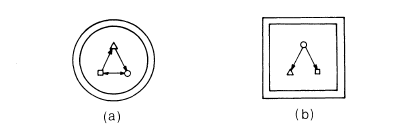
\includegraphics[width=0.6\textwidth]{imagenes/figura1.1.png}
    % Aquí va el código de TikZ para la Figura 1.2 (a->b, b->a, a<->b)
    \caption*{Fig. 1.2. Un sistema de dos componentes con tres posibles estructuras internas.}
\end{figure}

\vspace{0.5cm} % Pequeño espacio para separar del contenido anterior

{\fontsize{13}{15}\selectfont
\textbf{Ejemplo} Una molécula, un arrecife de coral, una familia y una fábrica son sistemas. Por otro lado, un conjunto de estados de una cosa y una colección de eventos, incluso si están ordenados, no son sistemas concretos. Símbolo: $\Sigma$.

Y ahora las tres características de cualquier sistema:

\textbf{DEFINICIÓN 1.2} Sea $\sigma' \in \Sigma$ un sistema concreto y $A \subset \mathcal{T}$ una clase de cosas. Entonces,

(i) la A-composición de $\sigma'$ en un momento dado $t$ es el conjunto de sus A-partes en $t$:
$$ \mathcal{C}_A(\sigma', t) = \{x \in A \mid x \subset \sigma'\}; $$

(ii) el A-entorno de $\sigma'$ en el momento $t$ es el conjunto de todas las cosas de clase $A$, que no son componentes de $\sigma'$, que actúan o son actuadas por componentes de $\sigma'$ en $t$:
$$ \mathcal{E}_A(\sigma', t) = \{x \in A \mid x \notin \mathcal{C}_A(\sigma', t) \land (\exists y)(y \in \mathcal{C}_A(\sigma', t) \land (x \triangleright y \lor y \triangleright x))\}; $$

(iii) la A-estructura (u organización) de $\sigma'$ en el momento $t$ es el conjunto de relaciones, en particular vínculos, entre los componentes de $\sigma'$, y entre estos y las cosas en el entorno de $\sigma'$, en $t$:
$$ \mathcal{S}_A(\sigma', t) = \{R_i \in B_A(\sigma', t) \cup \bar{B}_A(\sigma', t) \mid |B_A(\sigma', t)| \neq \emptyset \land 1 \le i \le n \}, $$
donde $B_A(\sigma', t)$ es el conjunto de relaciones de enlace (bonding relations), y $\bar{B}_A(\sigma', t)$ el de relaciones de no-enlace (non-bonding relations), definidas en $\mathcal{C}_A(\sigma', t) \cup \mathcal{E}_A(\sigma', t)$.

\textbf{Ejemplo} El sistema posible más simple está compuesto por dos cosas conectadas, $a$ y $b$, en un entorno agrupado en una sola cosa $c$. Es decir, $\mathcal{C}(\sigma') = \{a, b\}$, $\mathcal{E}(\sigma') = \{c\}$. Este sistema puede tener cualquiera de las siguientes estructuras internas: $a \triangleright b$, $b \triangleright a$, o $a \rightleftharpoons b$ (véase la Figura 1.2). (Estas son las estructuras internas concebibles. Pero algunas de ellas podrían no ser nomológicamente posibles, y mucho menos técnicamente factibles o incluso deseables.) En cuanto a
}

%------------------------------------------------------------------------------------------------
%PAGINA 8
\newpage
%%Faltan Figura Geometrica 8

\fancyhf{}
\fancyhead[l]{\thepage}
\begin{center}
{\fontsize{13}{16}\selectfont \textbf{CAPÍTULO 1}}
\end{center}
\vspace{0.5cm}

{\fontsize{13}{15}\selectfont
\begin{figure}[h!]
    \centering
    % Aquí se insertaría el código TikZ para la Figura 1.2
    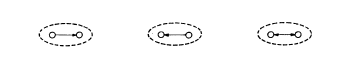
\includegraphics[width=0.6\textwidth]{imagenes/figura1.2.png}
    % Aunque no está en la imagen, sería una representación de a->b, b->a, y a<->b
    \caption*{Fig. 1.2. Un sistema de dos componentes con tres posibles estructuras internas.}
\end{figure}
las estructuras externas, pueden ser cualquiera de estas o sus uniones: $\{a \triangleright c\}$, $\{b \triangleright c\}$, $\{c \triangleright a\}$, $\{c \triangleright b\}$.

Un conocimiento exhaustivo de un sistema comprendería los siguientes puntos: (a) la composición, el entorno y la estructura del sistema; (b) la historia del sistema (particularmente si es un biosistema o un sociosistema); y (c) las leyes del sistema. Un conocimiento tan completo rara vez es alcanzable, particularmente con referencia a sistemas complejos. Pero para poder hablar de sistemas en absoluto, deberíamos conocer al menos su composición, su entorno y su estructura. Por lo tanto, podemos decir que el modelo constituido por la terna ordenada
$$ \sigma(\sigma, t) = \langle \mathcal{C}(\sigma, t), \mathcal{E}(\sigma, t), \mathcal{S}(\sigma, t) \rangle $$
es el **modelo mínimo** del sistema $\sigma$ en el momento $t$. Obviamente, este modelo cualitativo no será suficiente para propósitos cuantitativos, como predecir la tasa de formación o descomposición de un sistema. Por lo tanto, complementaremos el modelo mínimo anterior con un modelo cuantitativo que se presentará en la Sección 2.2. Sin embargo, antes de hacerlo, utilizaremos el modelo mínimo para aclarar una serie de cuestiones que a menudo son oscuras en la literatura sobre sistemas.

\subsection*{1.3. Más de lo Mismo}
Antes de continuar nuestro estudio de los sistemas y sus modelos, debemos asegurarnos de que el concepto de sistema concreto no esté ocioso, es decir, que algunas cosas sean sistemas mientras que otras no lo son. Que algunas cosas no son sistemas se deriva de la suposición de que existen cosas básicas o elementales, es decir, cosas sin partes (Vol. 3, Postulado 1.4). Y que otras cosas son sistemas se deriva de la hipótesis ontológica de que toda cosa —excepto el universo como un todo— actúa sobre, y es actuada por, otras cosas (Vol. 3, Postulado 5.10). En resumen, hemos demostrado el no trivial

\textbf{TEOREMA 1.1} (i) Existen sistemas concretos. (ii) Toda cosa es un componente de al menos un sistema.

Ciertamente, la identificación y el modelado de un sistema concreto pueden ser una tarea extremadamente difícil. Así, no siempre está claro cuál es la composición,
}

%------------------------------------------------------------------------------------------------
%PAGINA 9
\fancyhf{}
\fancyhead[r]{\thepage}
\newpage
\begin{center}
{\fontsize{13}{16}\selectfont \textbf{SISTEMA}}
\end{center}
\vspace{0.5cm}

{\fontsize{13}{15}\selectfont
... y, por lo tanto, también el entorno, de un sistema, particularmente si está fuertemente acoplado a otros sistemas —como es el caso de los sistemas económico y político de una sociedad. Sin embargo, este es un problema científico, no ontológico.

Nótese que las \textbf{acciones} y las \textbf{conexiones} correspondientes han sido definidas para \textbf{cosas}, no para \textbf{propiedades}. Estas últimas pueden ser interdependientes, pero no interactuantes. Es decir, la frase común 'Las propiedades $P$ y $Q$ interactúan' debe entenderse como "Las propiedades $P$ y $Q$ (de una cosa dada) son \textbf{interdependientes}", o "Las cosas con propiedad $P$ interactúan con las cosas con propiedad $Q$".

Las conexiones pueden ser permanentes o temporales, estáticas o dinámicas. En este último caso, a menudo se denominan \textbf{flujos} —de energía, como en la transferencia de calor; de materia, como en las migraciones; o de campos, como en una red de televisión. Si un flujo físico lleva información, la conexión se llama \textbf{informacional} y todo el sistema se denomina 'sistema de información'. Sin embargo, la distinción físico/informacional es de énfasis, no una dicotomía, ya que todo flujo de información se desplaza sobre algún flujo de energía. (Véase Apéndice A, Sec. 104.)

Nuestra definición del entorno de un sistema como el conjunto de todas las cosas acopladas con los componentes del sistema deja claro que se trata del \textbf{entorno inmediato}, no del entorno total, es decir, el conjunto de todas las cosas que no son parte del sistema. Excepto en la astronomía extragaláctica y en la cosmología, no estamos interesados en las transacciones de un sistema con el resto del universo, sino solo en aquella porción del mundo que ejerce una influencia significativa sobre la cosa de interés. Este \textbf{entorno inmediato} o \textbf{medio} es la célula en el caso de los cromosomas, el resto del organismo en el caso de un órgano, el ecosistema en el caso de un organismo, el sistema solar en el caso de una biosfera, y así sucesivamente. En otras palabras, el entorno inmediato de una cosa es la composición de su siguiente \textbf{supersistema}. (Más en la Sec. 104.)

Se dice que un sistema que ni actúa sobre, ni es actuado por, ninguna otra cosa es \textbf{cerrado}. En otras palabras, establecemos la

\textbf{DEFINICIÓN 1.3} Sea $\sigma'$ un sistema con entorno $\mathcal{E}(\sigma', t)$. Entonces $\sigma'$ es \textbf{cerrado} en $t$ si $\mathcal{E}(\sigma', t) = \emptyset$ — de lo contrario $\sigma'$ es \textbf{abierto}.

Dado que toda cosa, excepto el universo, interactúa con alguna otra cosa, inferimos el

\textbf{COROLARIO 1.1} El universo es el único sistema cerrado en todo momento.
}

%------------------------------------------------------------------------------------------------
%PAGINA 10
\newpage

\fancyhf{}
\fancyhead[l]{\thepage} 
\begin{center}
{\fontsize{13}{16}\selectfont \textbf{CAPÍTULO 1 }}
\end{center}
\vspace{0.5cm}

{\fontsize{13}{15}\selectfont
Esto se mantiene ya sea que el universo resulte ser espacialmente infinito o no, ya que el universo puede definirse como aquella cosa que tiene un \textbf{entorno vacío} (es decir, que es autocontenido).

Esto es en cuanto al concepto de cierre total. También necesitamos la noción de \textbf{cierre parcial}, o cierre relativo a una propiedad dada, ya que un sistema puede estar abierto en algunos aspectos y cerrado en otros. (Así, todos los sistemas están abiertos gravitacionalmente, pero algunos están cerrados eléctricamente, otros están cerrados al intercambio de materia, otros a las influencias culturales, y así sucesivamente.) Por lo tanto, establecemos la

\textbf{DEFINICIÓN 1.4} Sea $P$ una propiedad de un sistema $\sigma$ en un entorno $\mathcal{E}(\sigma, t)$. Entonces $\sigma$ es \textbf{abierto con respecto a} $P$ en $t$ si $P$ está relacionado, en $t$, con al menos una propiedad de las cosas en $\mathcal{E}(\sigma, t)$ — de lo contrario $\sigma$ es \textbf{cerrado} con respecto a $P$.

Comparando esta definición con la anterior, nos damos cuenta de que un sistema es cerrado si y solo si es cerrado en todos los aspectos.

Finalmente, algunos comentarios sobre el concepto de \textbf{estructura}. Nuestro uso de este concepto es común en matemáticas y en las ciencias sociales. Así, un famoso antropólogo afirma: para el bioquímico, un organismo "es un sistema complejamente integrado de moléculas complejas. El conjunto de relaciones mediante las cuales estas unidades están relacionadas es la \textbf{estructura orgánica}. Tal como se usan los términos aquí, el organismo no es en sí mismo una estructura; es una colección de unidades (células o moléculas) \textit{dispuestas en una estructura}, es decir, en un conjunto de relaciones; el organismo \textbf{tiene una estructura}" (Ratcliffe-Brown, 1935). Los biólogos usan 'estructura' a veces en el sentido anterior y en otras ocasiones como sinónimo de 'componente anatómico'. En este último caso, corren el riesgo de hablar de la estructura de una estructura.

A veces es útil distinguir la \textbf{estructura interna} de un sistema de su \textbf{estructura externa}. La primera es el subconjunto de la estructura total formado por las relaciones (en particular, las conexiones) entre los componentes del sistema. Y la estructura externa es, por supuesto, el complemento de la estructura interna a la estructura total. Aunque distintas, la estructura interna y la externa son \textbf{interdependientes}. Así, la estructura interna de una molécula, lejos de ser una propiedad permanente e intrínseca de la molécula, depende críticamente de su estructura externa, es decir, de las interacciones entre la molécula y su medio (por ejemplo, el solvente).

Otra distinción que vale la pena hacer es la que existe entre la \textbf{estructura total} y la \textbf{estructura espacial}, o el conjunto de relaciones espaciales entre las partes de una cosa. (\textbf{La estructura o configuración espacial no debe confundirse con la forma}. La gran mayoría de los sistemas en el universo, es decir, los átomos de hidrógeno y helio, carecen de forma. Los sistemas sociales tampoco tienen forma, aunque
}